% === C03 - Interrupciones basicas ===
% David Alejandro Gonzalez Marquez
% dmarquez@dc.uba.ar / fokerman@gmail.com
% https://github.com/fokerman/Orga2Course

\documentclass[aspectratio=169]{beamer}
% \documentclass[handout]{beamer}

% % % Packages
\usepackage[sfdefault]{AlegreyaSans}
\usepackage{inconsolata}
\usepackage{multicol}
\usepackage{multirow}
\usepackage[spanish]{babel}
\usepackage[utf8]{inputenc}
\usepackage{enumerate}
\usepackage{color}
\usepackage{xcolor}
\usepackage[absolute,overlay]{textpos}
  \setlength{\TPHorizModule}{1mm}
  \setlength{\TPVertModule}{1mm}
\usepackage{framed}
\usepackage{mfirstuc} % para poner en mayusculas la primer letra
\usepackage{xspace} % para crear espacios en comandos 
\usepackage{pbox}
\usepackage{tikz}
\usepackage{mathabx}

% % % Beamer config
\usetheme{Pittsburgh}
\usecolortheme[rgb={1,0.48,0.0}]{structure}
\setbeamercolor{block title}{fg=white,bg=verdeuca}
\xdefinecolor{verdeuca}{rgb}{0.0,0.48,0.54}
\xdefinecolor{naranjauca}{rgb}{1,0.48,0.0}
\setbeamercolor{palette quaternary}{fg=white,bg=verdeuca}
\setbeamertemplate{title page}[default][colsep=-4bp, rounded=true] % remove title shadow
\setbeamertemplate{frametitle}[default][colsep=-2bp, shadow=false] % remove frame title shadow
\setbeamertemplate{navigation symbols}{} % remove navigation symbols
\beamertemplatenavigationsymbolsempty

% % % Colors
\definecolor{AzulClaro}{rgb}{.31,.506,.741}
\definecolor{Gris}{gray}{0.8}
\definecolor{Celeste}{rgb}{.255,.41,.884}
\definecolor{Rojo}{rgb}{1, 0, 0}
\definecolor{a}{rgb}{0.0, 0.53, 0.74}
\definecolor{r}{rgb}{0.89, 0.0, 0.13}
\definecolor{v}{rgb}{0.0, 0.5, 0.0}
\definecolor{y}{rgb}{0.0, 0.5, 0.5}
\definecolor{rojo}{HTML}{F1521B}
\definecolor{verde}{HTML}{80CD29}
\definecolor{amarillo}{HTML}{FABC09}
\definecolor{azul}{HTML}{00ADF1}

% % % Rename
\newcommand{\tab}[0]{\hspace{15pt}}

% % % Blocks
\setbeamercolor{block body}{fg=black, bg=black!10}
\setbeamercolor{block title}{fg=black, bg=black!20}
\setbeamercolor{coloredboxstuffNaranja}{fg=naranjauca,bg=black!10} %% PARA LOS BOX
\setbeamercolor{coloredboxstuffVerde}{fg=verdeuca,bg=black!10} %% PARA LOS BOX

% % % Start

\title{\Huge Interrupciones Básicas}
\subtitle{Programación de Sistemas Operativos}
      
\author{David Alejandro González Márquez}
\institute{Departamento de Computación\\
Facultad de Ciencias Exactas y Naturales\\
Universidad de Buenos Aires}
\date{}

\begin{document}

\frame[plain]{\titlepage}

\begin{frame}
    \only<2>{\frametitle{Usted estabá aquí}}
    \only<3>{\frametitle{Usted estará aquí}}
    \only<1>{\frametitle{Usted ...}}
    \begin{textblock}{100}(45,2) \only<2->{\includegraphics[scale=0.52]{img/usted_esta_aqui-layer1.pdf}} \end{textblock}
    \begin{textblock}{100}(46,2) \only<3->{\includegraphics[scale=0.52]{img/usted_esta_aqui-layer2.pdf}} \end{textblock}
    \begin{textblock}{100}(46,2) \only<1->{\includegraphics[scale=0.52]{img/usted_esta_aqui-layer3.pdf}} \end{textblock}
\end{frame}

\begin{frame}
    \frametitle{IDT - Interruption Descriptor Table}
    \Large
    \begin{itemize}
    \item[-] Soporta 256 tipos de interrupciones
    \pause
    \vspace{0.2cm}
    \item[-] Se utiliza una tabla denominada \texttt{IDT}
    \pause
    \vspace{0.2cm}
    \item[-] La \texttt{IDT} almacena \textbf{descriptores de interrupción}
    \pause
    \vspace{0.2cm}
    \item[-] El registro \texttt{IDTR} almacena la dirección de la \texttt{IDT}
    \end{itemize}
\end{frame}

%\subsection{IDTR}

\begin{frame}
    \frametitle{IDTR and IDT}
    \begin{figure}
    \centering
        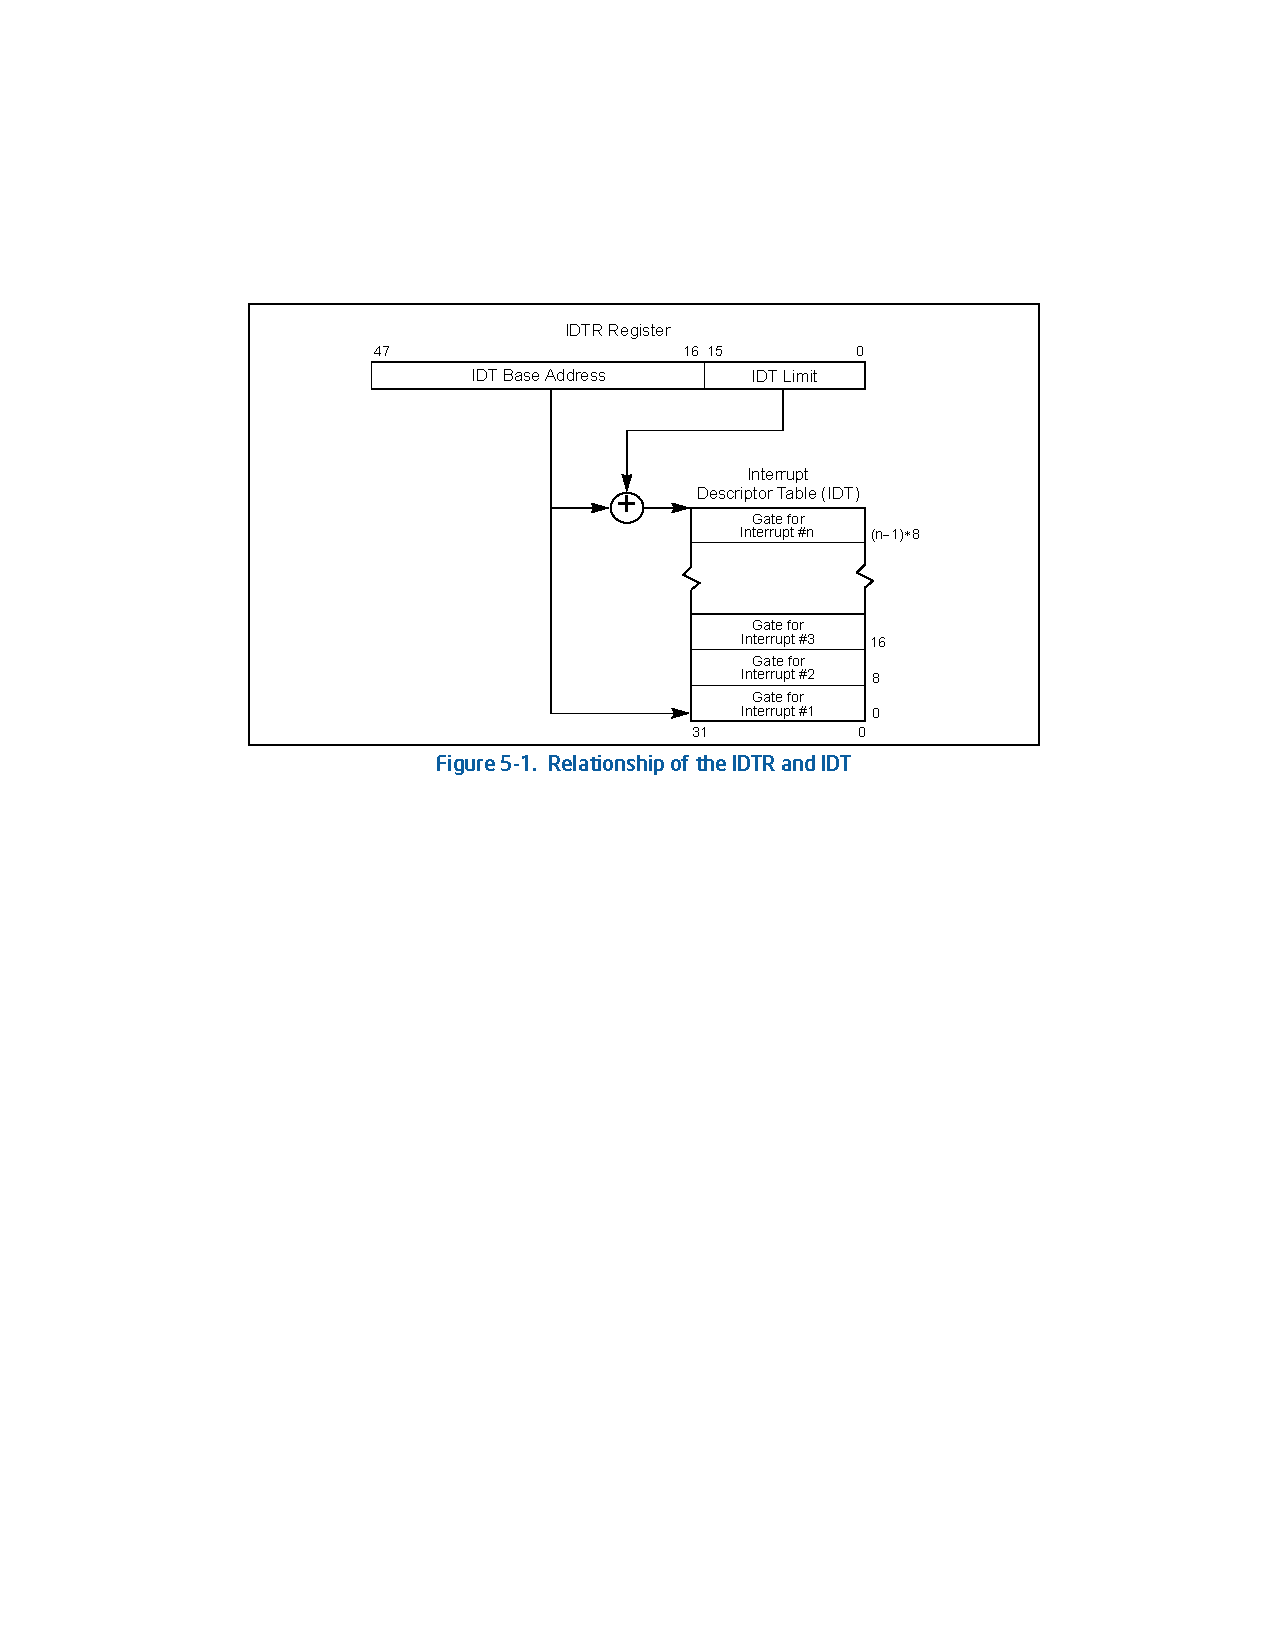
\includegraphics[scale=0.8]{img/idtr_and_idt}
    \end{figure}
\end{frame}

\begin{frame}
\frametitle{Gate Descriptors}
    \vspace{-0.7cm}
    \begin{table}
    \centering
        \begin{tabular}[h]{cc}
    {\vtop{\null\hbox{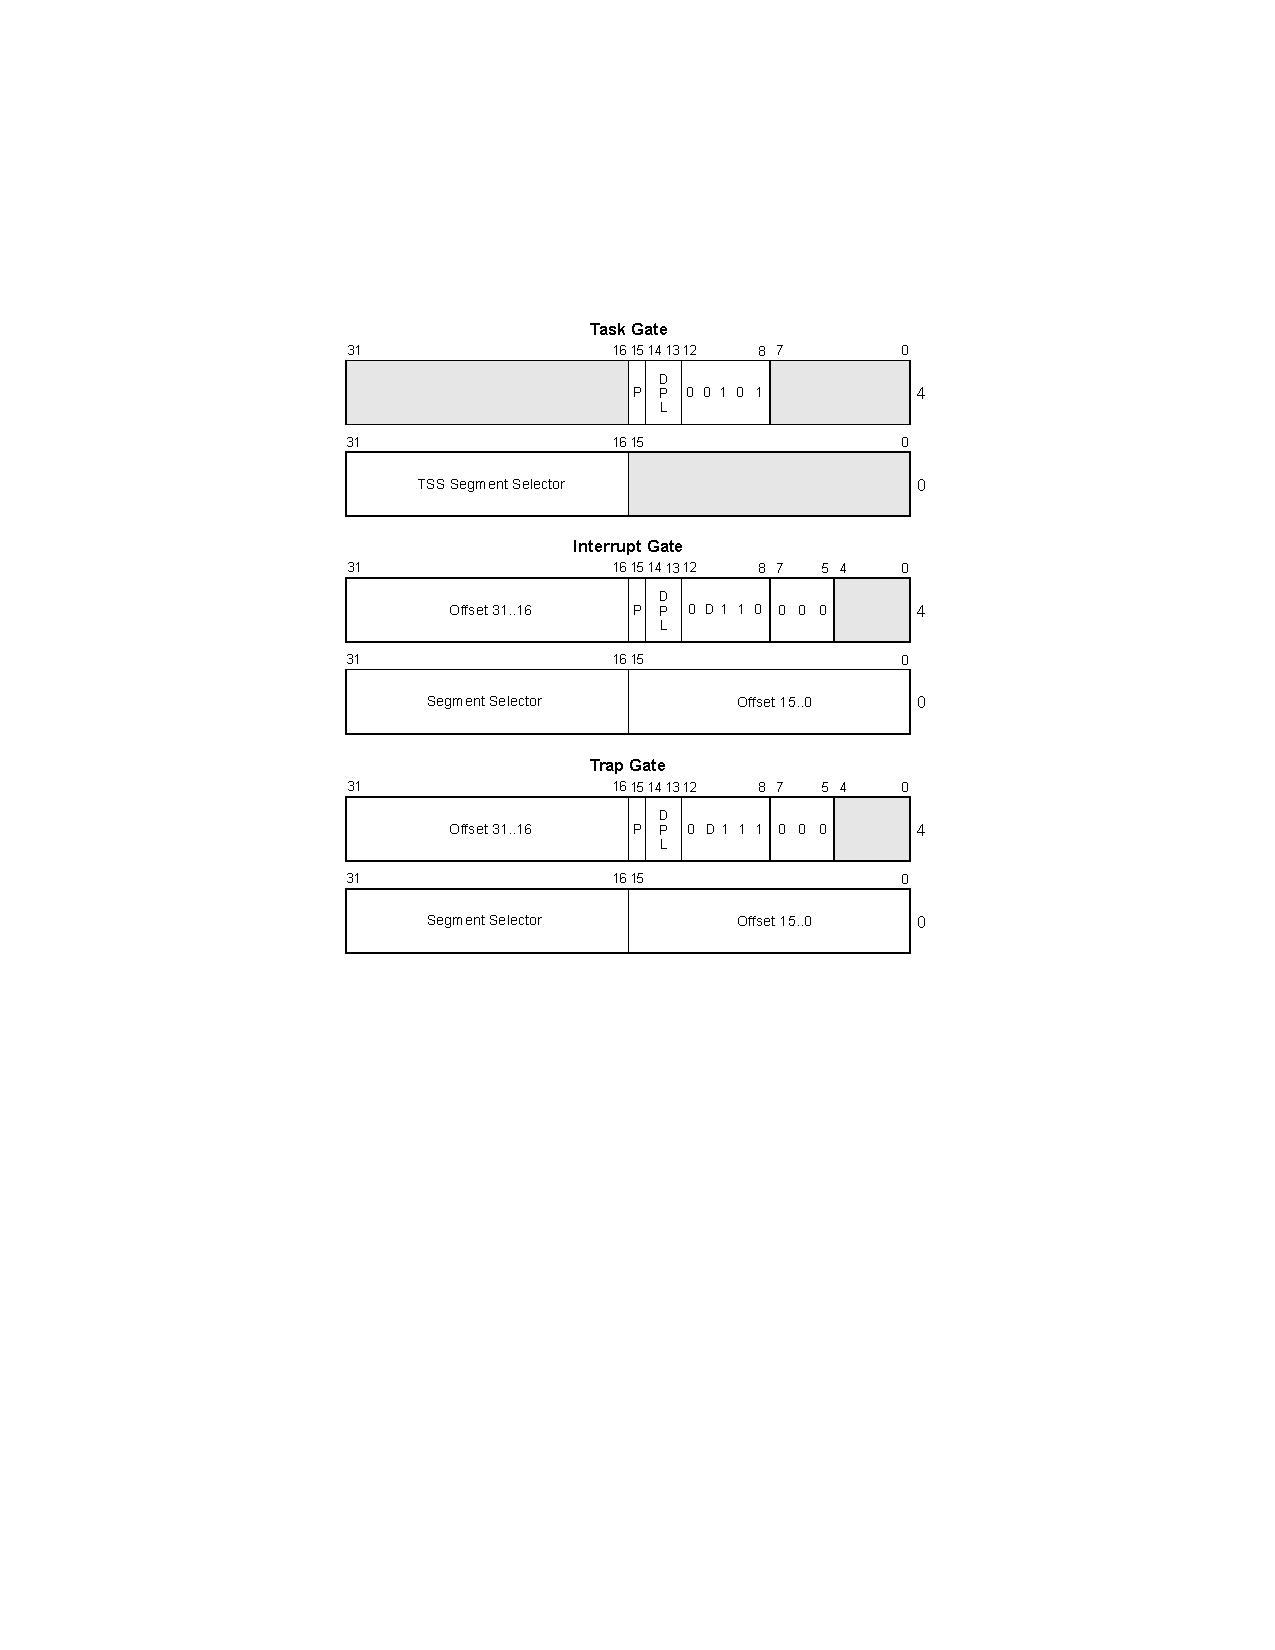
\includegraphics[scale=0.66]{img/gate_descriptors_solo}}}}
    &
    {\vtop{\null\hbox{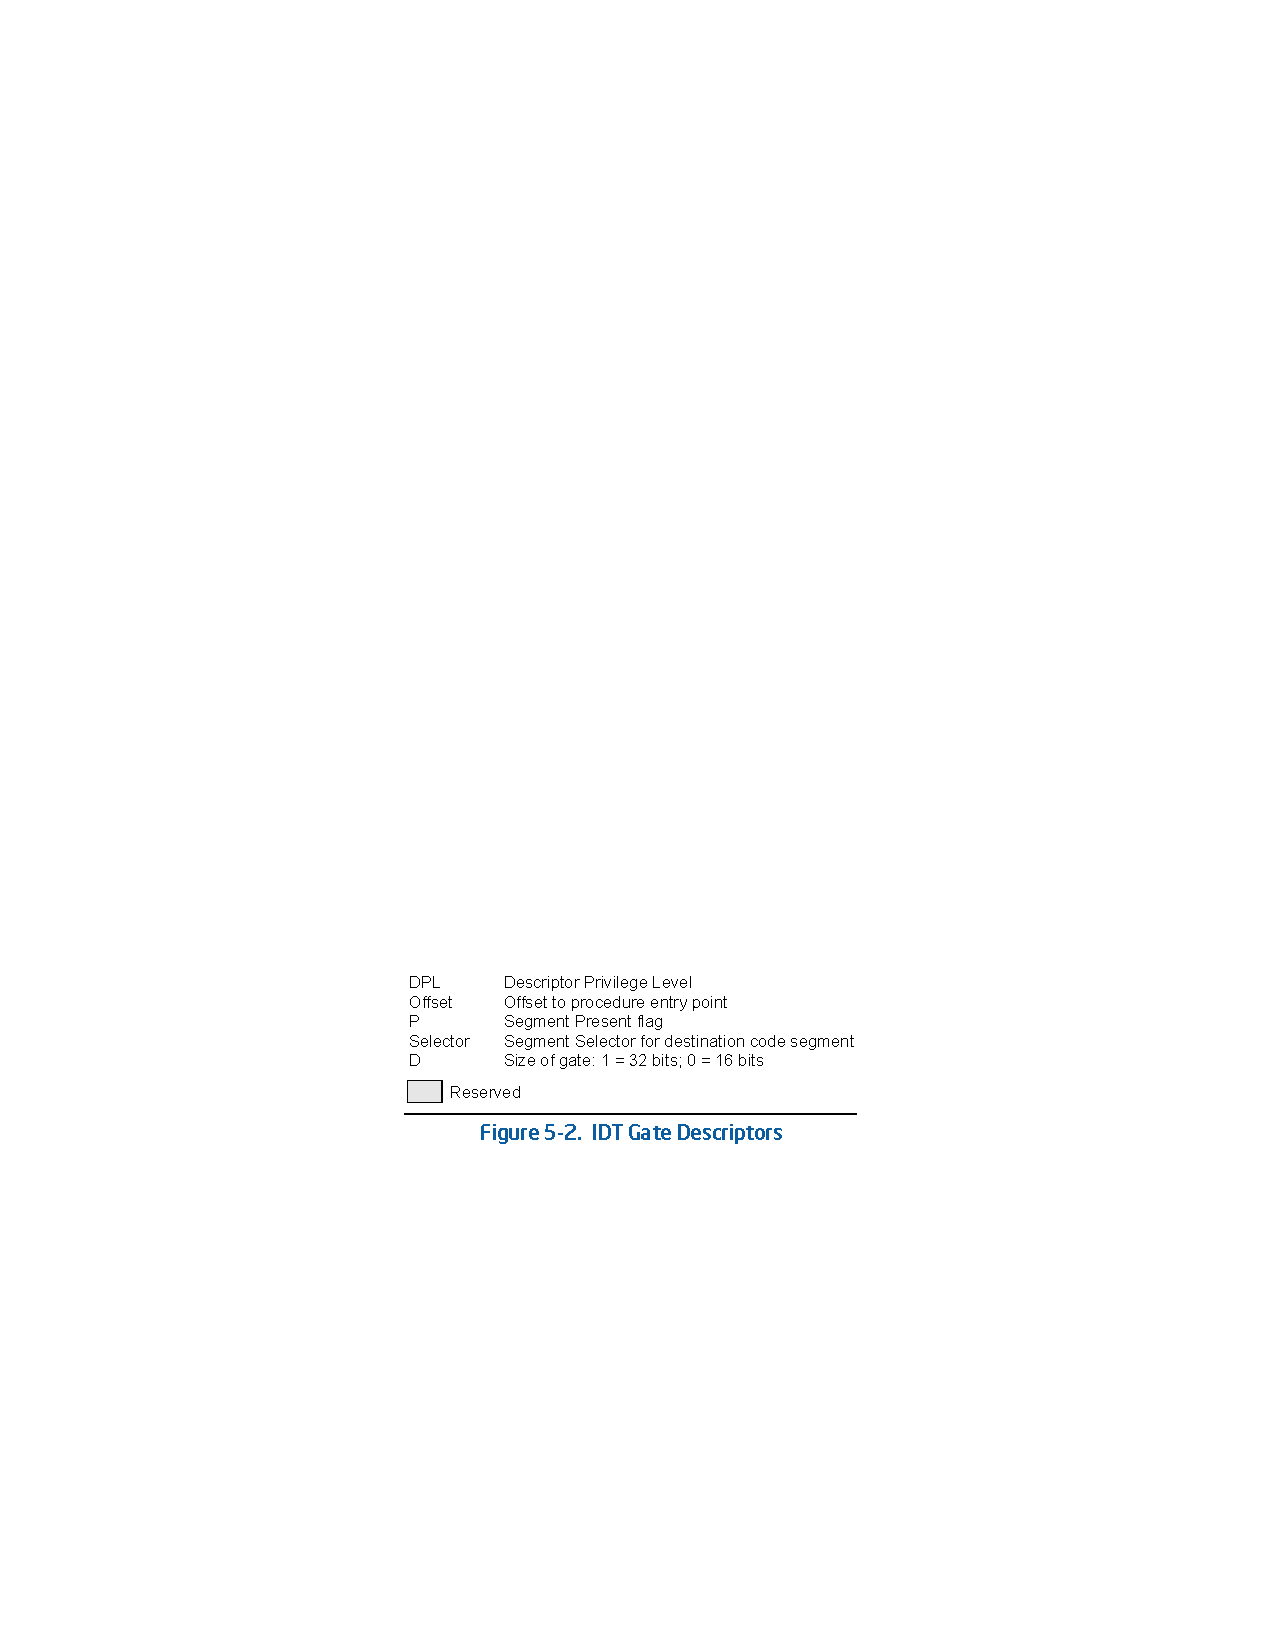
\includegraphics[scale=0.55]{img/gate_descriptors_desc}}}}
    \\
        \end{tabular}
    \end{table}
    \begin{textblock}{65}(95,30)
    \begin{itemize}
    \small
     \item<2->[-]  \textcolor{verdeuca}{\emph{Task Gate}:} Inicia una tarea para anteder\\ la interrupción.
     \item<3->[-]  \textcolor{verdeuca}{\emph{Interrupt Gate}:} Detene interrupciones y atiende la interrupción.
     \item<4->[-]  \textcolor{verdeuca}{\emph{Trap Gate}:} No detene interrupciones y atiende la interrupción.
    \end{itemize}
    \begin{itemize}
    \small
     \item<5->[] Vamos a utilizar \textbf{Interrupt Gate} para atender nuestras interrupciones.
    \end{itemize}
    \end{textblock}
\end{frame}

\begin{frame}
    \frametitle{Interrupt Procedure Call}
    \begin{textblock}{100}(5,12)
            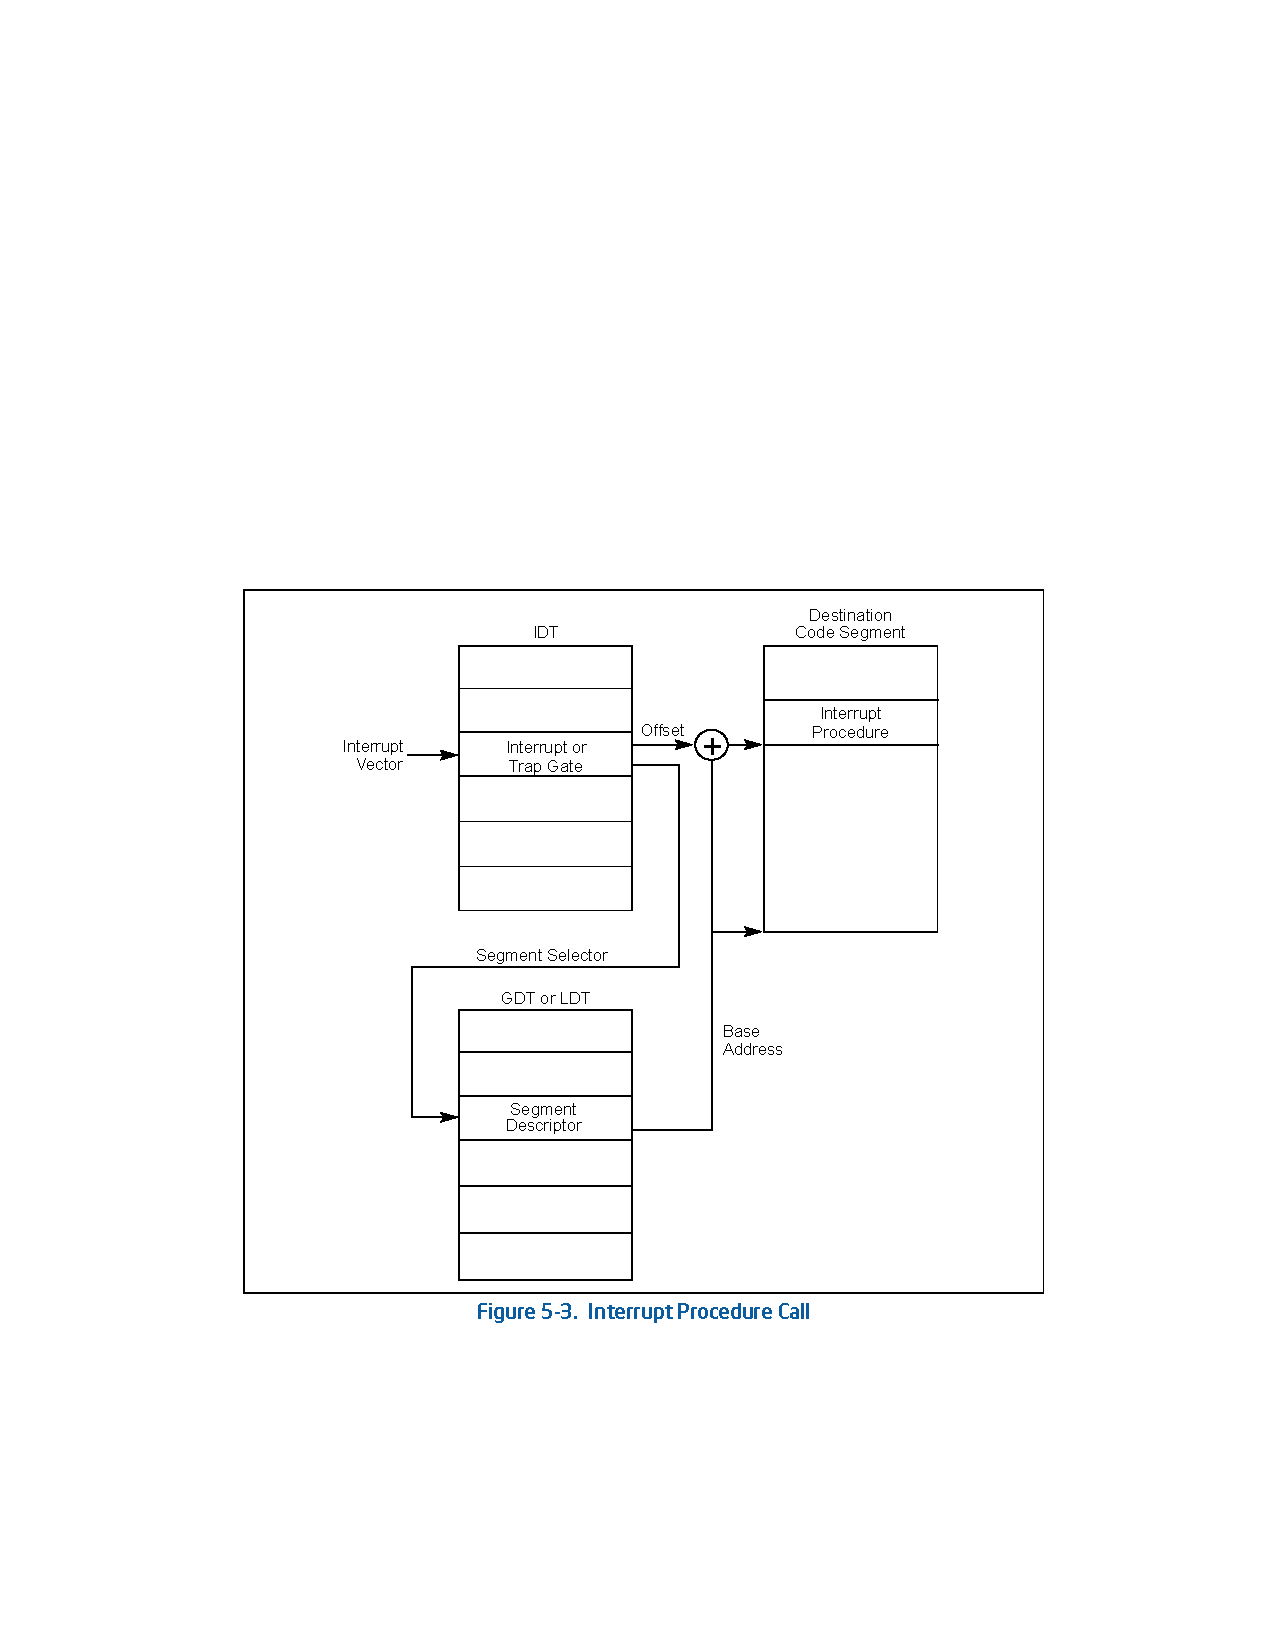
\includegraphics[scale=0.60]{img/procedure_call} 
    \end{textblock}
    \begin{textblock}{70}(87,12)
        \begin{enumerate}
        \small
        \setlength\itemsep{0.4cm}
        \item<2->[-] Llega el vector de interrupción (índice) y se atiende según indique su entrada en la IDT.
        \item<3->[-] Se obtiene el \textcolor{verdeuca}{\texttt{segment}} y se lo busca en la GDT
        \item<4->[-] Se obtiene la base del segmento, y junto al \textcolor{verdeuca}{\texttt{offset}} se calcula la dirección de la rutina de atención de interrupciones.
        \item<5->[-] Se comienzá a ejecutar la rutina en la dirección \textcolor{verdeuca}{\texttt{segment:offset}}
        \end{enumerate}
    \end{textblock}
\end{frame}

\begin{frame}
    \frametitle{Interrupt Task Switch}
    \begin{textblock}{100}(5,12)
            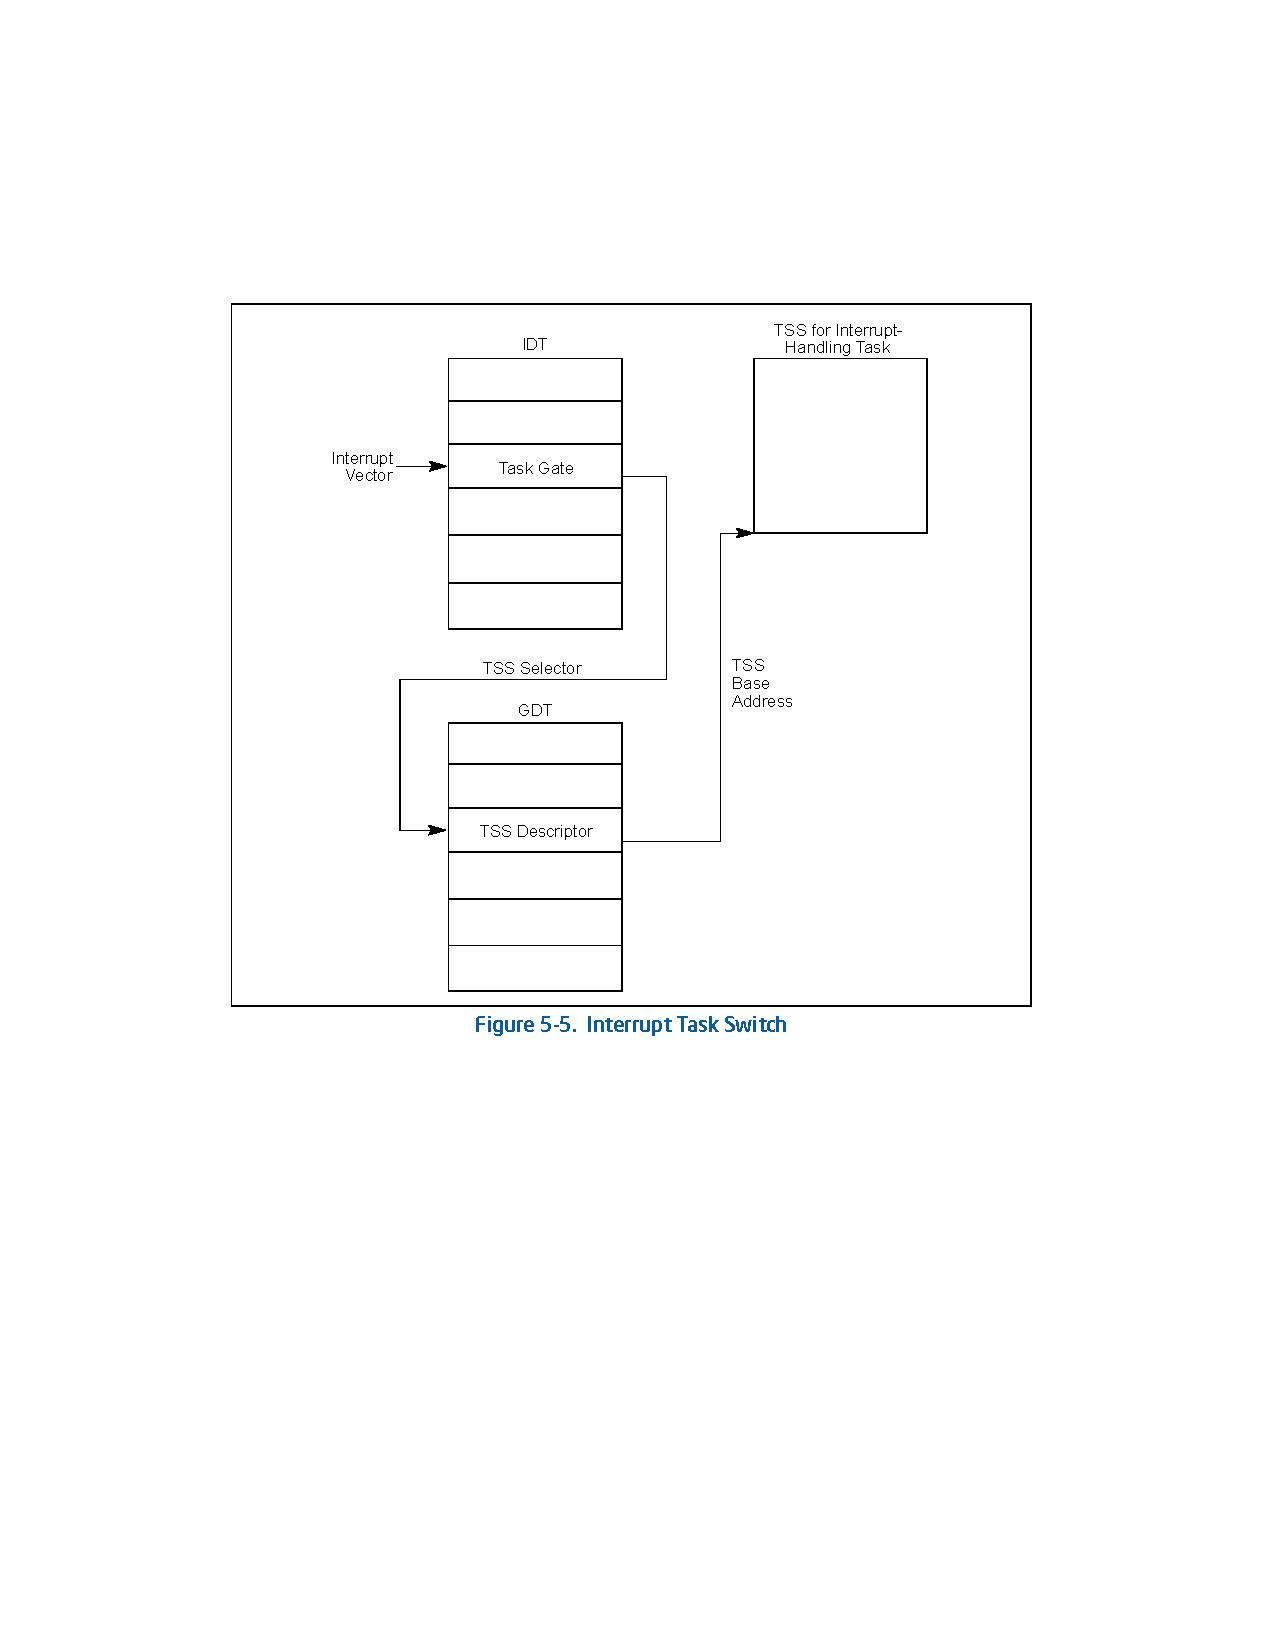
\includegraphics[scale=0.60]{img/interrupt_task} 
    \end{textblock}
    \begin{textblock}{70}(87,12)
        \begin{enumerate}
        \small
        \setlength\itemsep{0.4cm}
        \item<2->[-] Llega el vector de interrupción (índice) y se atiende según indique su entrada en la IDT.
        \item<3->[-] Se obtiene el \textcolor{verdeuca}{\texttt{segment}} y se lo busca en la GDT
        \item<4->[-] Se obtiene el contexto de ejecución de la tarea asociada a la entrada en la GDT.
        \item<5->[-] Se comienzá a ejecutar la tarea, intercambiandola con la tarea actual.
        \end{enumerate}
    \end{textblock}
\end{frame}

\begin{frame}
    \frametitle{Tipos de Interrupciones}
    \begin{itemize}
    \setlength\itemsep{0.3cm}
    \item[-] \textbf{Fault}\\ Excepción que puede corregirse permitiendo al programa
    retomar la ejecución de esa instrucción sin perder continuidad.
    El procesador guarda en la pila la dirección de la instrucción
    que produjo la falla.
    \pause
    \item[-] \textbf{Traps}\\ Excepción producida inmediatamente a continuación de 
    una instrucción de trap. Algunas permiten al procesador retomar la
    ejecución sin perder continuidad. Otras no. El procesador guarda en
    la pila la dirección de la instrucción a ejecutarse luego de la
    instrucción trapeada.
    \pause
    \item[-] \textbf{Aborts}\\ Excepción que no siempre puede determinar la
    instrucción que la causá, ni permite recuperar la ejecución de
    la tarea que la causá. Reporta errores severos de hardware o
    inconsistencias en tablas del sistema.
    % Faults - A fault is an exception that can generally be corrected and that, once \vspace{-0.7cm}	 
    %corrected, allows the program to be restarted with no loss of continuity. When a 	 
    %fault is reported, the processor restores the machine state to the state prior to 	 
    %the beginning of execution of the faulting instruction. The return address (saved 	 
    %contents of the CS and EIP registers) for the fault handler points to the faulting 	 
    %instruction, rather than to the instruction following the faulting instruction. 	 
    % Traps - A trap is an exception that is reported immediately following the 	 
    %execution of the trapping instruction. Traps allow execution of a program or task 	 
    %to be continued without loss of program continuity. The return address for the 	 
    %trap handler points to the instruction to be executed after the trapping 	 
    %instruction. 	 
    % Aborts - An abort is an exception that does not always report the precise
    %location of the instruction causing the exception and does not allow a restart of
    %the program or task that caused the exception. Aborts are used to report severe
    %errors, such as hardware errors and inconsistent or illegal values in system
    %tables.
    \end{itemize}
\end{frame}

\begin{frame}
    \frametitle{Interrupt Table}
    \vspace{-0.7cm}
    \begin{figure}
    \centering
    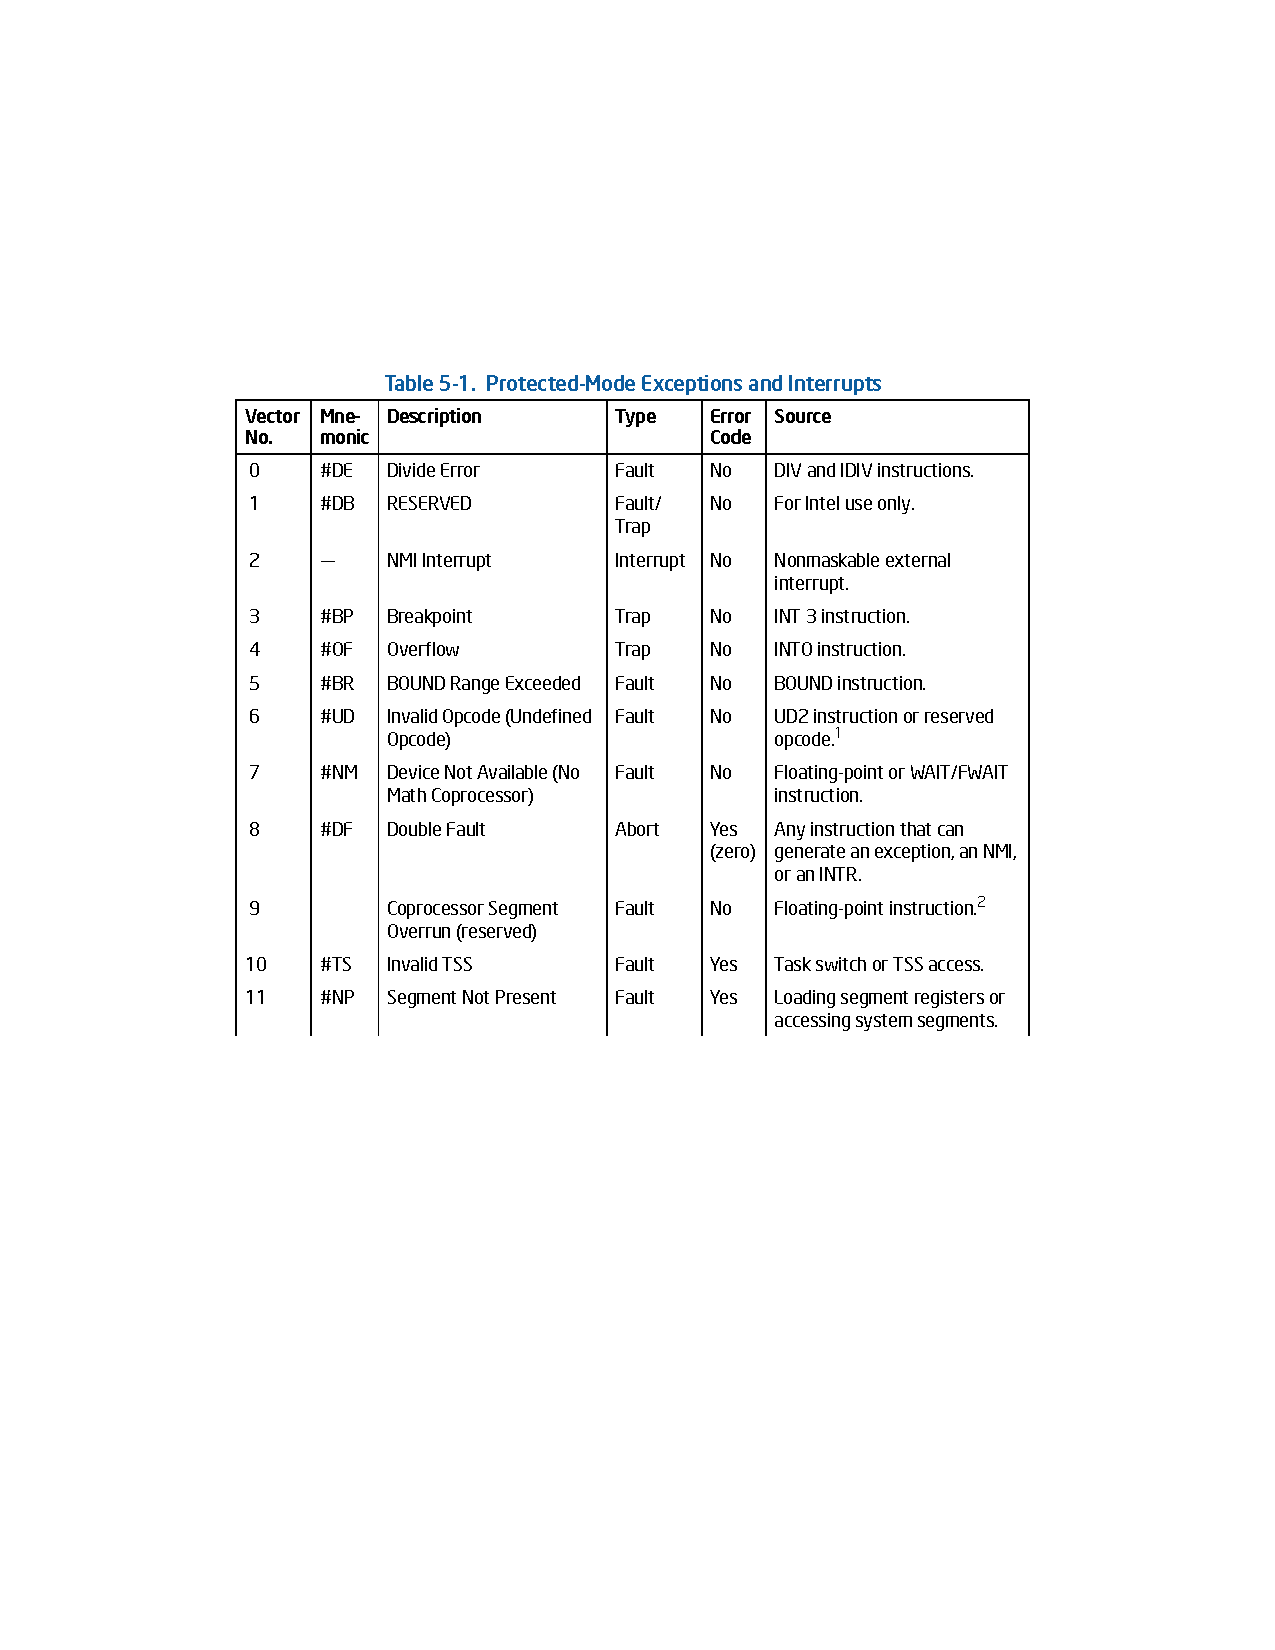
\includegraphics[scale=0.65]{img/tabla_int1_1}
    \end{figure}
\end{frame}

\begin{frame}    
    \frametitle{Interrupt Table}
    \vspace{-0.6cm}
    \begin{figure}
    \centering
    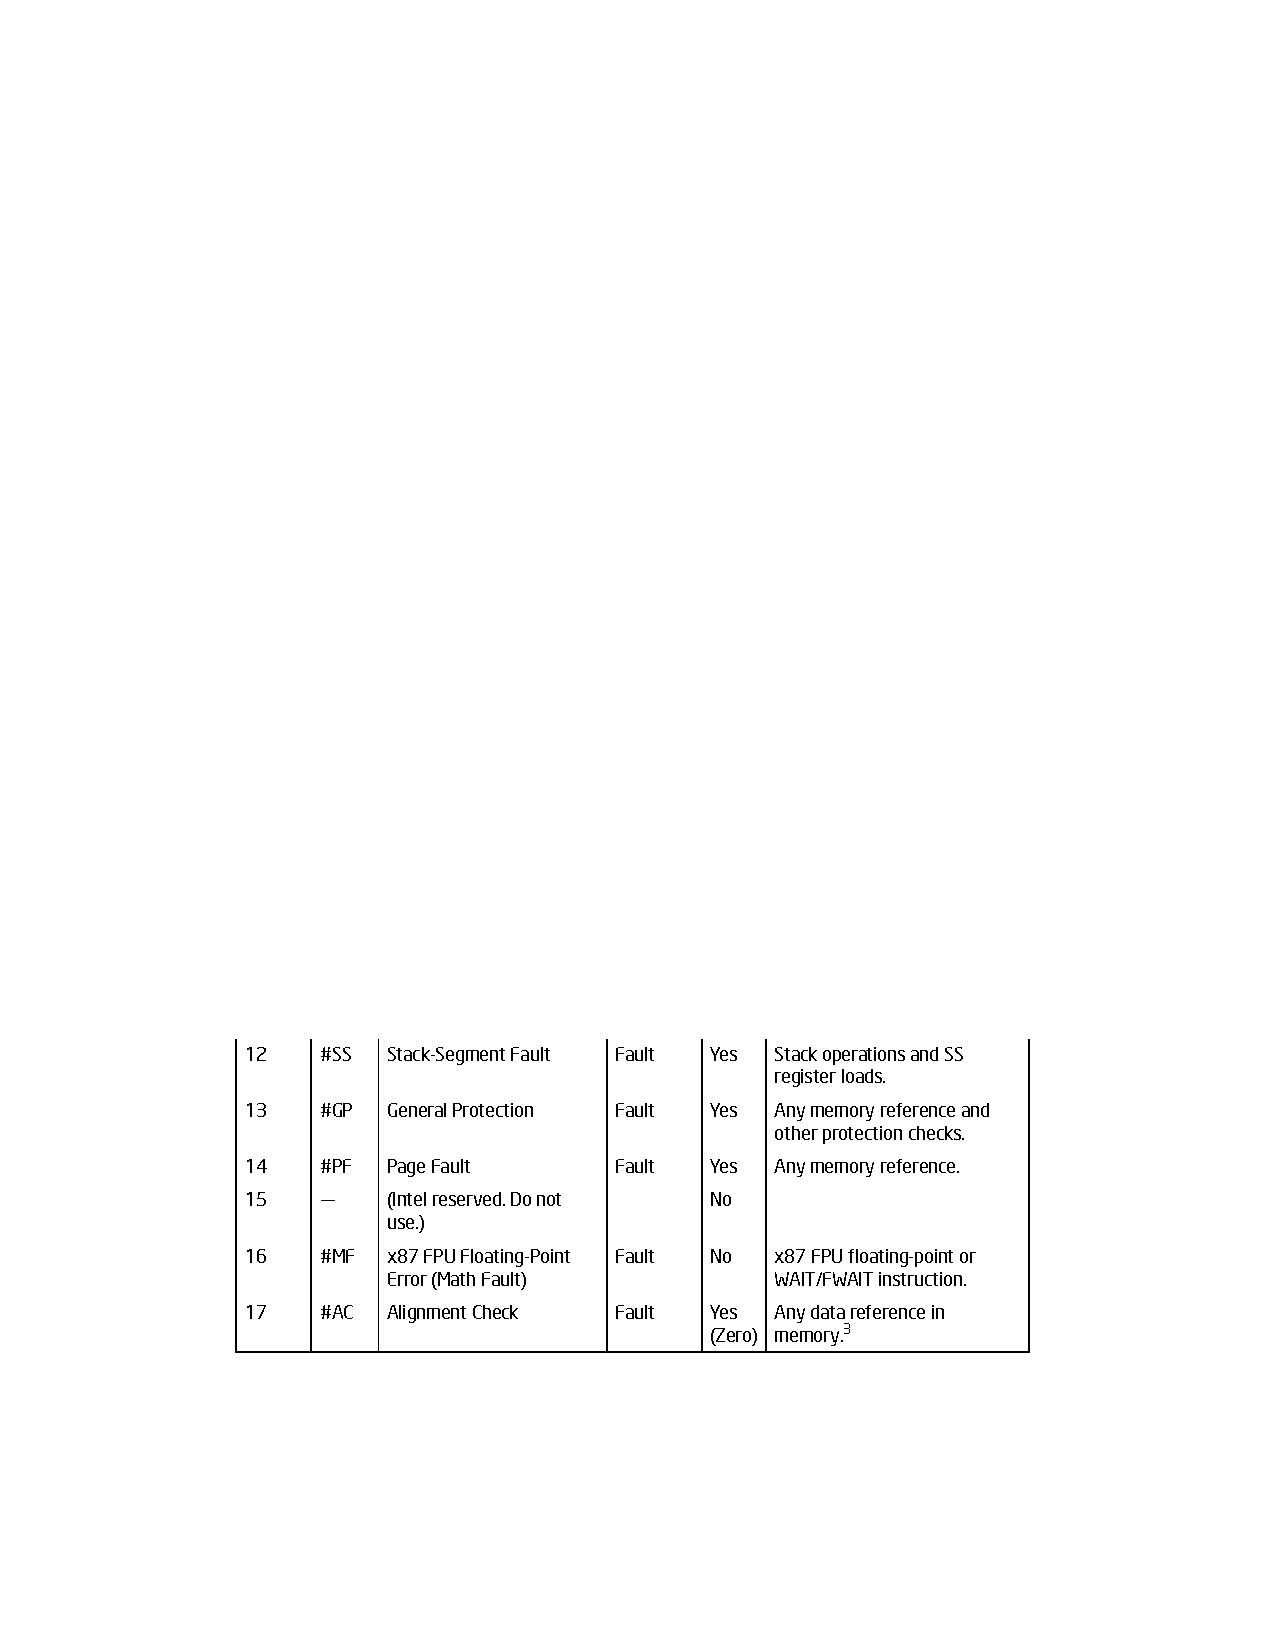
\includegraphics[scale=0.65]{img/tabla_int1_2}
    \end{figure}
    \vspace{-0.3cm}
    \begin{figure}
    \centering
    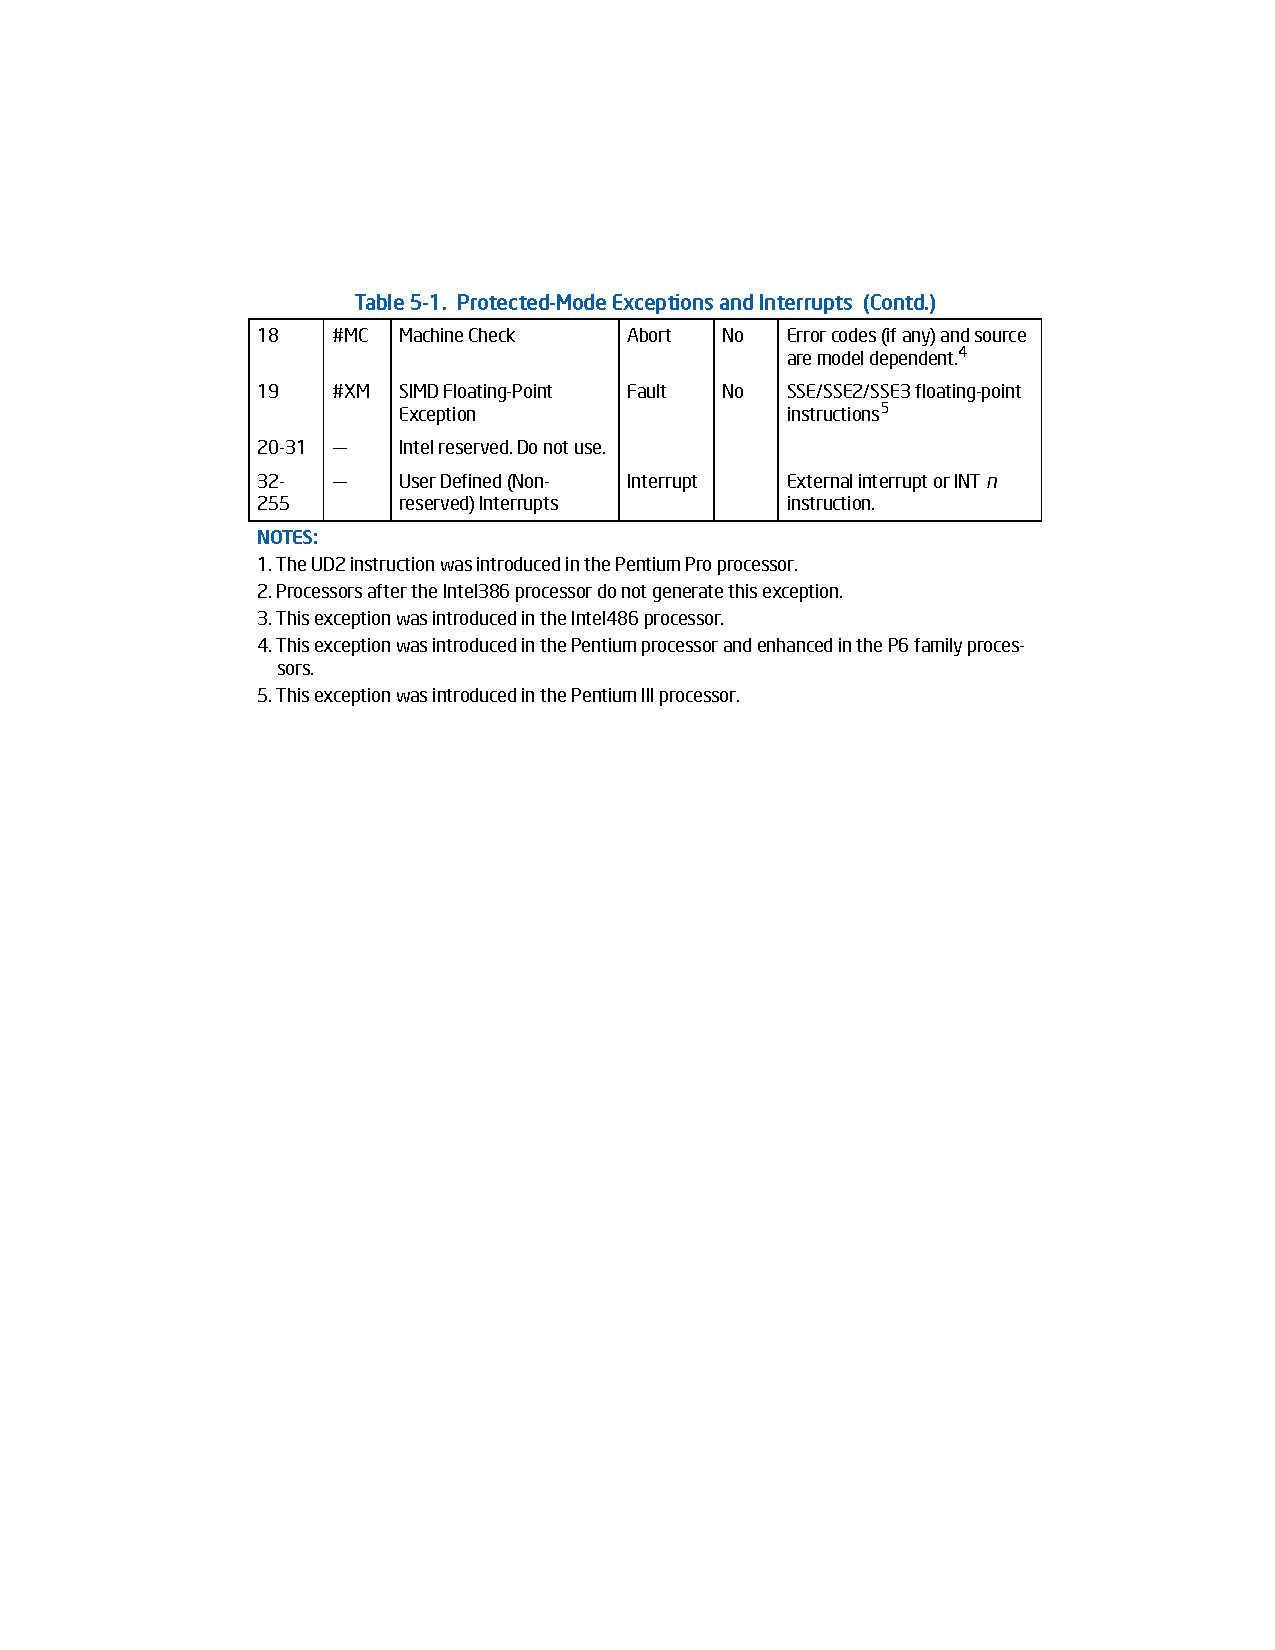
\includegraphics[scale=0.65]{img/tabla_int2}
    \end{figure}
\end{frame}

\begin{frame}
    \frametitle{Stack}
    \vspace{-0.6cm}
    \begin{figure}
    \centering
    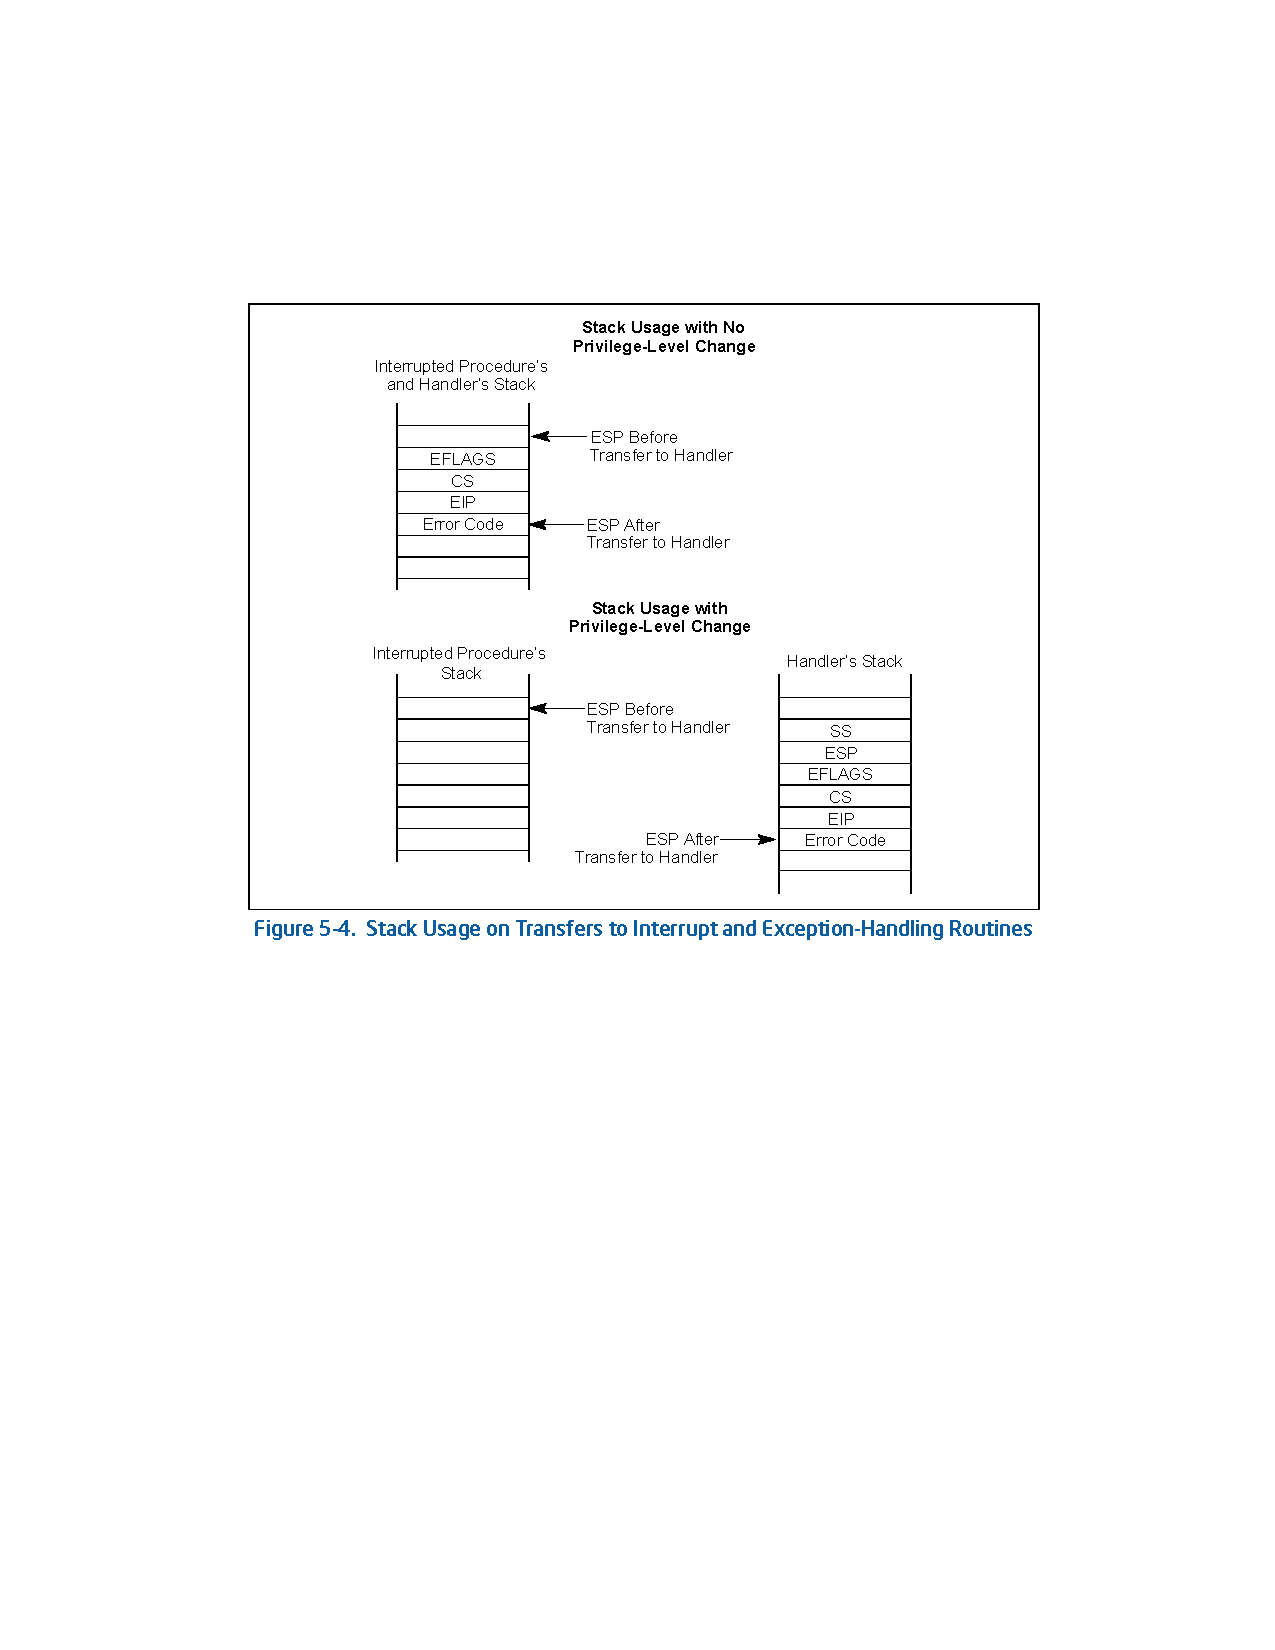
\includegraphics[scale=0.72]{img/stack}
    \end{figure}
\end{frame}

\begin{frame}
    \frametitle{Error Code}
    \begin{figure}
    \centering
    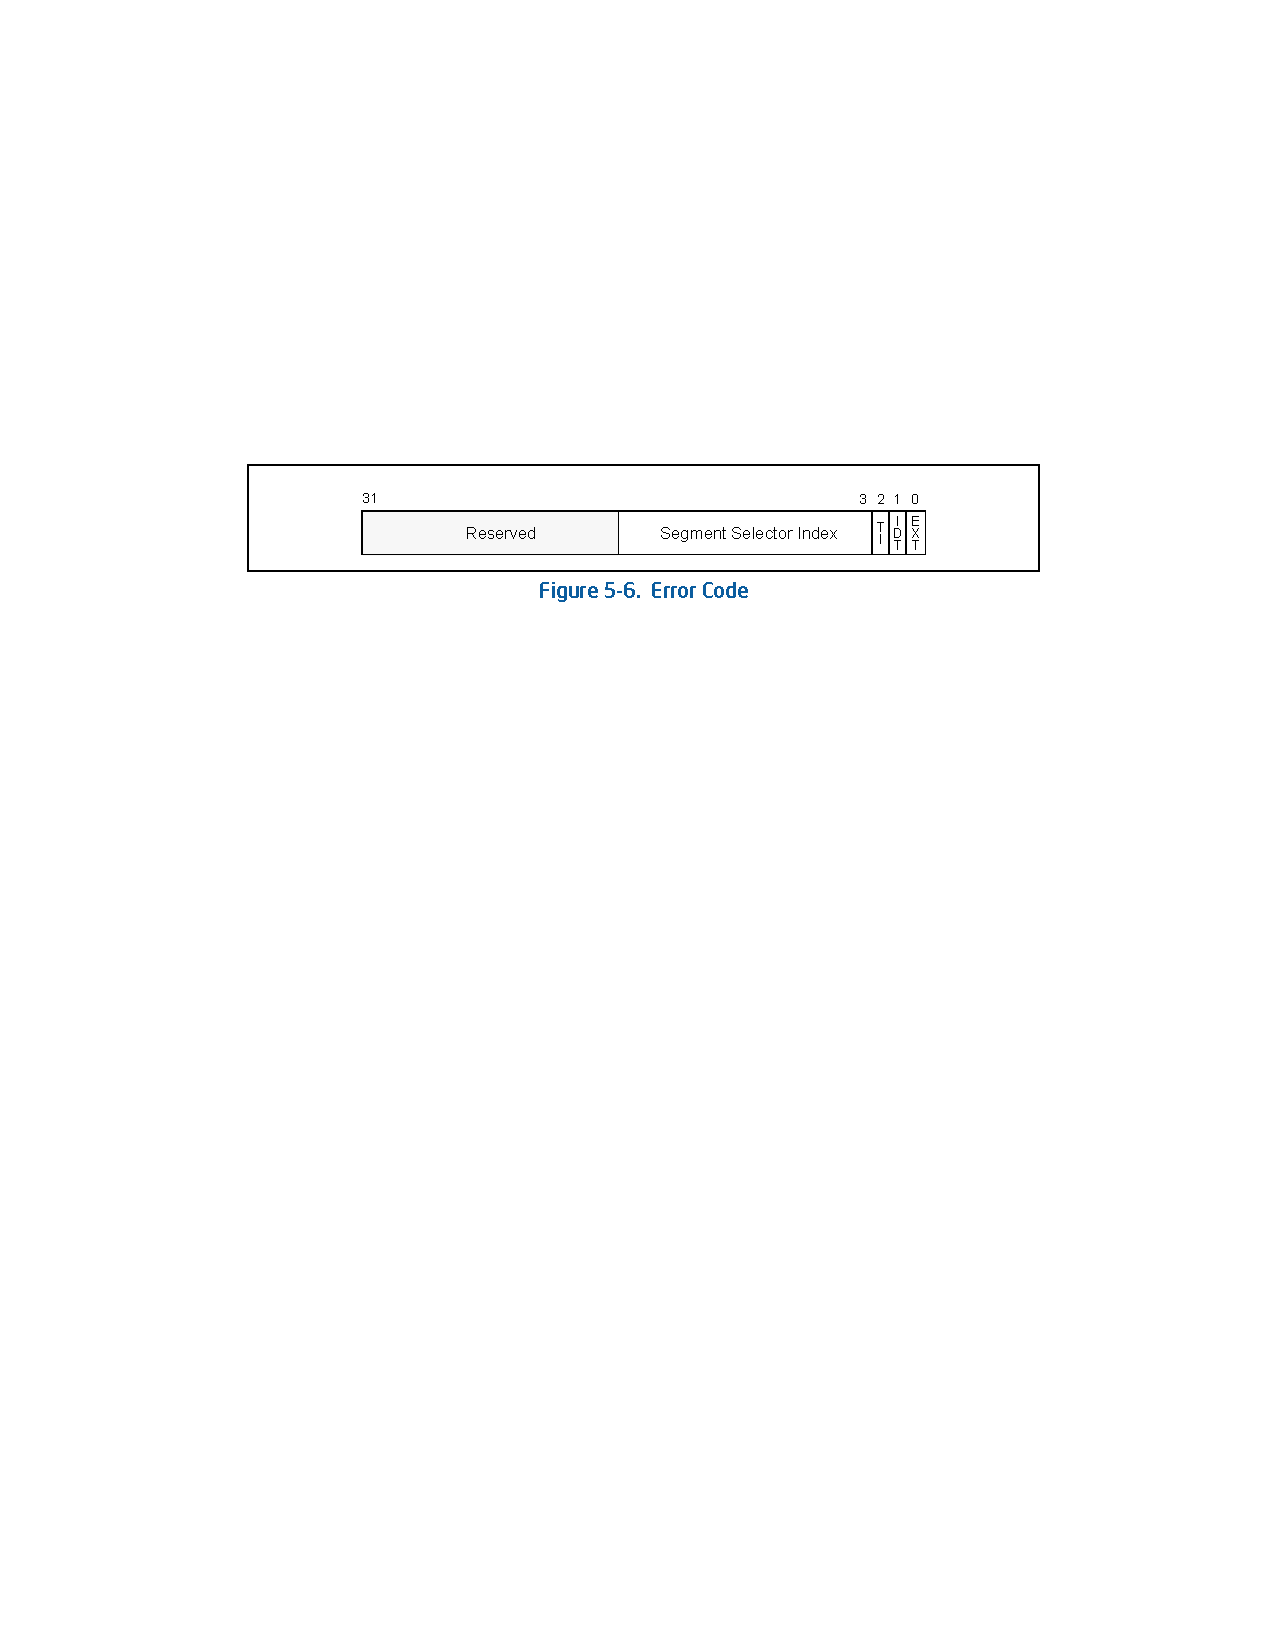
\includegraphics[scale=0.8]{img/error_code}
    \end{figure}
    \vspace{-0.3cm}
    \begin{itemize}
    \setlength\itemsep{0.1cm}
    \pause
    \item[-] \textbf{EXT}: (External Event)\\
    Se setea para indicar que la excepción ha sido causada por un evento externo al procesador.
    \pause
    \item[-] \textbf{IDT}: (Descriptor Location)\\
    Cuando está seteado indica que el campo Segment Selector Index se refiere a un descriptor de puerta en la IDT. Cuando est en cero indica que dicho campo se refiere a un descriptor en la GDT o en la LDT de la tarea actual.
    \pause
    \item[-] \textbf{TI}: (GDT/LDT)\\
    Tiene significado cuando el bit anterior est en cero. Indica a que tabla de descriptores corresponde el selector del campo Indice. (GDT=0 , LDT=1)
    % (idntico significado que en el selector de segmento)
    %- EXT 	External event (bit 0)  When set, indicates that an event external 	 
    %to the program, such as a hardware interrupt, caused the exception. 	 
    %- IDT 	Descriptor location (bit 1)  When set, indicates that the index 	 
    %portion of the error code refers to a gate descriptor in the IDT; when 	 
    %clear, indicates that the index refers to a descriptor in the GDT or the
    %current LDT.
    %- TI GDT/LDT (bit 2)  Only used when the IDT flag is clear. When set,
    %the TI flag indicates that the index portion of the error code refers to
    %a segment or gate descriptor in the LDT; when clear, it indicates that
    %the index refers to a descriptor in the current GDT.
    \end{itemize}
\end{frame}

\begin{frame}[fragile]
    \frametitle{Archivos}
    \begin{enumerate}
    \item \Large \texttt{idt.h}\\ \normalsize Descripción de las estructuras
    \vspace{0.5cm}
    \pause
    \item \Large \texttt{idt.c}\\ \normalsize Estructura de la \texttt{IDT} con cada una de sus entradas
    \end{enumerate}
    \begin{itemize}
    \setlength\itemsep{0.3cm}
    \pause
    \item[-] \verb|idt_entry idt[255] = { ... };|
    \pause
    \item[-] \texttt{IDT\_ENTRY(}\textcolor{verdeuca}{\texttt{numero}}\texttt{)}\\
    Permite declarar una entrada en la \texttt{IDT}, para la utilizar el handler de nombre \textcolor{naranjauca}{\texttt{\_isr}}\textcolor{verdeuca}{\texttt{numero}}
    \pause
    \item[-] \texttt{void init\_idt()}\\ Función llamada desde el kernel para inicializar las entradas en la \texttt{IDT}
    \end{itemize}
\end{frame}

\begin{frame}[fragile]
    \frametitle{Estructuras}
    \begin{itemize}
    \item[-] \textcolor{verdeuca}{Struct de descriptor de IDT}
    \begin{verbatim}
    typedef struct str_idt_descriptor {
        unsigned short idt_length;
        unsigned int idt_addr;
    } __attribute__((__packed__)) idt_descriptor;
    \end{verbatim}
    \vspace{0.3cm}
    \item[-] \textcolor{verdeuca}{Struct de una entrada de la IDT}
    \begin{verbatim}
    typedef struct str_idt_entry_fld {
            unsigned short offset_0_15;
            unsigned short segsel;
            unsigned short attr;
            unsigned short offset_16_31;
    } __attribute__((__packed__, aligned (8))) idt_entry;
    \end{verbatim}
    \end{itemize}
\end{frame}

\begin{frame}
\frametitle{Rutinas de Atención de Interrupción}
    \begin{block}{Cómo manejar correctamente una interrupción}
    \begin{enumerate}
    \setlength\itemsep{0.7cm}
        \item Preservar los registros que vayamos a romper \pause $\rightarrow$ \alert{\emph{¡la interrupción debe ser transparente!}}
        \pause
        \item Realizar la tarea correspondiente a la interrupción
        \pause
        \item Restaurar los registros
        \pause
        \item Retornar de la interrupción
    \end{enumerate}
    \end{block}
\end{frame}

\begin{frame}[fragile]
    \frametitle{Bibliografía: Fuentes y material adicional}
    \begin{itemize}
    \item Convenciones de llamados a función en x86: \\
    \url{https://en.wikipedia.org/wiki/X86_calling_conventions}
    \item Notas sobre System V ABI: \\
    \url{https://wiki.osdev.org/System_V_ABI}
    \item Documentación de NASM: \\
    \url{https://nasm.us/doc/}
    \item Artículo sobre el flag \texttt{-pie}: \\
    \url{https://eklitzke.org/position-independent-executables}
    \item Documentación de System V ABI: \\
    \url{https://uclibc.org/docs/psABI-x86_64.pdf}
    \item Manuales de Intel: \\
    \url{https://software.intel.com/en-us/articles/intel-sdm}
    \end{itemize}
\end{frame}

\begin{frame}[plain]
    \begin{center}
    \vspace{2cm}
    \huge ¡Gracias!\\
    \vspace{2cm}
    \normalsize Recuerden leer los comentarios al final de \\ este video por aclaraciones o fe de erratas.
    \end{center}
\end{frame}

\end{document}

%\tiny
%\begin{table}
%	\centering
%		\begin{tabular}{|c|c|l|l|l|l|}
%		\hline5
%		Vec. & Mne & Description & Type & Error  & Source \\ 
%		No.  &     &             &      & Code & \\
%		\hline
%		0 & \#DE & Divide Error & Fault & No & DIV and IDIV instructions. \\
%		1 & \#DB & RESERVED & Fault/ Trap & No & For Intel use only. \\
%		2 & - & NMI Interrupt & Interrupt & No & Nonmaskable external \\
%		  &   &               &           &    & interrupt. \\
%		3 & \#BP & Breakpoint & Trap & No & INT 3 instruction. \\
%		4 & \#OF & Overflow & Trap & No & INTO instruction. \\
%		5 & \#BR & BOUND Range Exceeded & Fault & No & BOUND instruction. \\
%		6 & \#UD & Invalid Opcode & Fault & No & UD2 instruction or \\
%			&   &               &           &    & reserved opcode.1 \\
%		7 & \#NM & Device Not Available & Fault & No & Floating-point \\
%		&   &               &           &    & or WAIT/FWAIT instruction. \\
%		 	&      & (No Math Coprocessor) &  &  &  \\
%		8 & \#DF & Double Fault & Abort & Yes & Any instruction \\
%		&   &               &           & (zero)   &  that can generate an exception, \\
%		&   &               &           &    &  an NMI, or an INTR. \\
%		9 & - & Coprocessor Segment Overrun & Fault & No & Floating-point instruction.2 \\
%		10 & \#TS & Invalid TSS & Fault & Yes & Task switch or TSS access. \\
%		11 & \#NP & Segment Not Present & Fault & Yes & Loading segment registers \\
%		&   &               &           &    & or accessing system segments. \\
%		12 & \#SS & Stack-Segment Fault & Fault & Yes & Stack operations and SS \\
%		&   &               &           &    & register loads. \\
%		13 & \#GP & General Protection & Fault & Yes & Any memory reference and \\
%		&   &               &           &    & other protection checks. \\
%		14 & \#PF & Page Fault & Fault & Yes & Any memory reference. \\
%		15 &  & (Intel reserved. Do not use.) & & No & \\
%		16 & \#MF & x87 FPU Floating-Point Error & Fault & No & x87 FPU floating-point or \\
%		&   &               &           &    &  WAIT/FWAIT instruction. \\
%		17 & \#AC & Alignment Check & Fault & Yes (Zero) & Any data reference in memory.3 \\
%		18 & \#MC & Machine Check & Abort & No & Error codes (if any) and source \\
%		&   &               &           &    &  are model dependent.4 \\
%		19 & \#XM & SIMD Floating-Point Exception & Fault & No & SSE/SSE2/SSE3 \\
%		&   &               &           &    & floating-point instructions5 \\
%		20-31 & - &         &           &    & Intel reserved. Do not use. \\
%		\hline
%		32-255 & - & User Defined (Non-reserved) & Interrupt &  & External interrupt or \\
%		&   &               &           &    & INT n instruction. \\
%		\end{tabular}
%\end{table}
